\chapter{はじめに} \label{intro}
\pagenumbering{arabic}  %% ページ番号をアラビア数字に変更

高等学校での物理学の授業では、実験は重要である。
Holubova~\cite{holubova_2019}は、実験室での作業は理論的な概念を検証する最も重要な方法であり、生徒は実験を通してどのような現象が起きるかを確認することができると述べている。

しかし実際は、生徒全員が実験を経験しているわけではない。林らは、2014年に大学生を対象に物理実験の経験を調査した~\cite{2015KJ00010038066}。これによると、力学分野で最も基本的な「運動の法則」に関する実験経験は60\%であった。また、斜方投射の基本的な問題である「モンキーハンティング~(\ref{monkey_hunting})」に関する実験は10\%に満たない。
この理由としては、実験用の装置の準備や測定が難しいことや、実験を行うのに時間を要することが考えられる。

\begin{figure}[b]

\noindent\rule{\linewidth}{0.4pt}

\begin{quote}
小球を、位置 $(0, 0)$ から初速 $v_0$、 仰角 $\theta$ で発射したところ、位置 $(l, h)$ から自由落下してくる物体に衝突した。 $\tan \theta$ の満たすべき条件を求めよ。ただし、重力加速度の大きさを $g$ とする。
\end{quote}

\centering
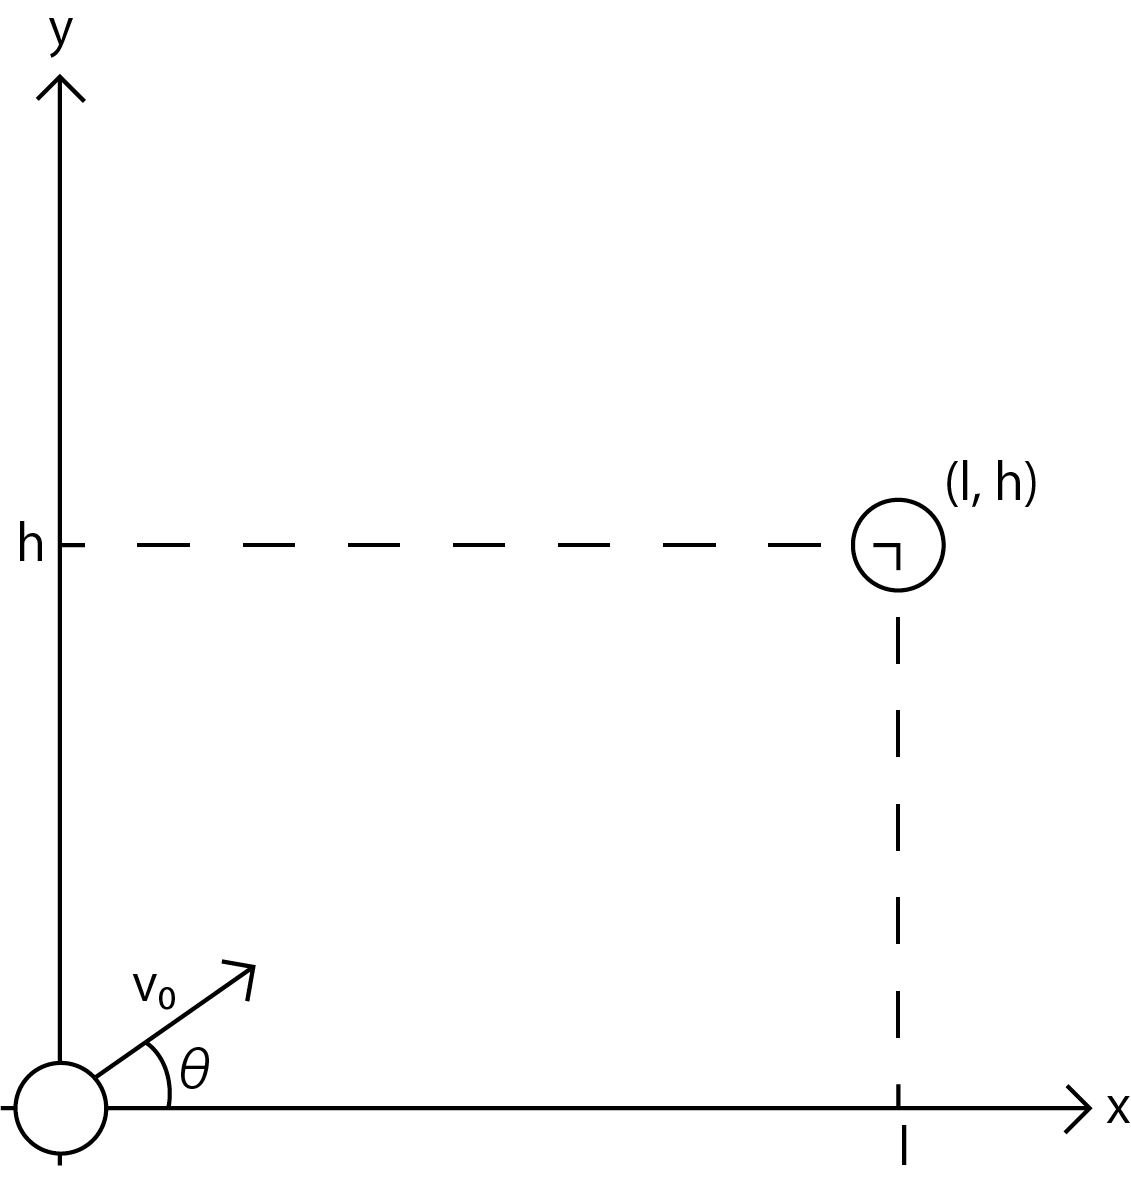
\includegraphics[width=0.3\linewidth]{work/monkey_hunting.png}
\caption{モンキーハンティング} \label{monkey_hunting}
\end{figure}

そこで実験の代替として近年利用されているのが、物理実験のシミュレータである。シミュレータを用いることで、実験と同様の学習効果を得ることができる。Ajredini~\cite{ajredini_real_2014} は、既存の物理実験シミュレータである PhET~\cite{perkins_phet_2006} を用いる授業と実際に実験を行う授業を実施し、テストを行った。その結果、シミュレーションによって得られる知識と実際の実験によって得られる知識の間には有意な差はないと結論づけた。


% TODO: 既存のシミュレータは〇〇という点で不十分である。思いついたら
しかし、既存のシミュレータでは不十分な点が存在する。学習者が理論を学習するとき、物理法則やそれを前提とした運動を方程式を通して学習する。
図~\ref{symbol_based}は実際に生徒が解く問題の例
%TODO: \cite{}
である。学習者は教科書等で学習した物理法則を方程式の形で利用し、結果も方程式の形で表現される。一方既存のシミュレータである PhET では、図~\ref{numeral_based}のように速度や質量、位置のような物理量を数値でしか確認できず、描画されている物理系がどのような方程式によって表現されているのかわからない。

\begin{figure}[b]
\noindent\rule{\linewidth}{0.4pt}

\small{\textbf{(問題)} 静止している質量 $m$ の物体に大きさ $F$ の力をかけ続ける。$t$ 秒後の速さを求めよ。}

\small{\textbf{(解答)} 物体の加速度を $a$ とする。運動方程式より $ma~=~F$ $\therefore~a~=~\dfrac{F}{m}$ 。等加速度運動の公式より $v~=~at~=~\dfrac{F}{m}t$\\
答え: $\dfrac{F}{m}t$}

\caption{方程式の計算例} \label{symbol_based}
\end{figure}

\begin{figure}[thb]
\centering
\includegraphics*[width=0.9\linewidth]{figure/PhET_example.png}
\caption{PhET のシミュレーション例} \label{numeral_based}
\end{figure}

そこで本研究では、物理系を定義できるシミュレータである \simname~(\simnamealt) を提案する。学習者は \simname で系内の物体をそのパラメータとともに定義し、その物体の運動を表す方程式を立式する。この際学習者は、次元の異なる物理量の和が存在する不正な方程式を立式すると警告されるなど、正しい物理系を作成するための補助を受ける。シミュレーションを実行すると、定義した物理系に基づいて数値計算がなされ、物体の運動が可視化される。さらに、 \simname には現実の運動を正しく表現した動作例が存在し、学習者が参考にすることができる。

\simname の利点は、
現実の運動を確認できるだけでなく、学習者が定義した方程式と現実の物理法則に従う物体の運動の対応を理解できるという点である。既存のシミュレータはツール側が物理系を全て提供し、学習者はパラメータを指定するだけである。一方 \simname では、学習者は動作例と比較しながら物理系を定義することで、現実の運動がどのような方程式で表されるものなのか理解できる。

なお、\simname は実際にシミュレーションを表示する部分以外は未実装であるが、\ref{idea}章で説明するアイデアは\ref{implementation}章に記す方針で実装が可能であると考えている。

本論文の構成は以下の通りである。
第\ref{related}章で、既存のシミュレータとそれを用いた実例について紹介する。
第\ref{idea}章で、\simname のアイデアを説明する。
第\ref{implementation}章で、\simname の実装について説明する。
% 第\ref{evaluation}章で、\simname の評価方法を提案する。
第\ref{conclusion}章で、まとめと今後の展望について述べる。
